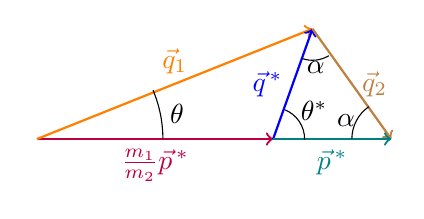
\begin{tikzpicture}
\draw [->, thick, purple](-3,-0.5) node (v1) {} -- (0,-0.5) node [midway, below] {$\frac{m_1}{m_2}\vec{p}^{\,*}$};
\draw [->, thick, orange] (v1.center) -- (0.5,0.9) node [midway, above] {$\vec{q}_1$};
\draw [->, thick, blue](0,-0.5) node (v3) {} -- (0.5,0.9)node [midway, left] {$\vec{q}^{\,*}$};
\draw [->, thick, brown] (0.5,0.9) -- (1.5,-0.5) node [midway, right] {$\vec{q}_2$};
\draw[->, thick, teal] (v3.center) -- (1.5,-0.5)node [midway, below] {$\vec{p}^{\,*}$};
\draw (-1.525,0.12) arc (22.7989:0:1.6)node [midway, right] {$\theta$};
\draw (0.1472,-0.1281) arc (68.4061:-1.2:0.4)node [midway, above right=-3] {$\theta^*$};
\draw (1,-0.5) arc (180:124.8:0.5)node [midway, left=-3] {$\alpha$};
\draw (0.3685,0.5222) arc (-109.1914:-58.8:0.4)node [midway, below=-3] {$\alpha$};
%\node at (-0.6,-1.3) {Choque elástico $\implies p^*=q^*$};

\end{tikzpicture}